\documentclass[main]{subfiles}


\begin{document}
\newpage
\section{Introduction}

\subsection{Motivation}
Deep-learning, a brain-inspired weak form of artificial intelligence, allows the training of large \textbf{artificial neuronal networks} (ANNs) that, like humans, can learn real-world tasks such as recognizing objects in images. The origins of deep hierarchical learning can be traced back to early neuroscience research by Hubel and Wiesel in the 1960s, who first described the neuronal processing of visual inputs in the mammalian neocortex. Similar to their neocortical counterparts, ANNs seem to learn by interpreting and structuring the data provided by the external world. However, while on specific tasks such as playing (video) games, deep ANNs outperform humans (Minh et al, 2015, Silver et al., 2018), ANNs are still not performing on par when it comes to recognizing actions in movie data and their ability to act as generalizable problem solvers is still far behind of what the human brain seems to achieve effortlessly. Moreover, \textbf{biological neuronal networks} (BNNs) seem to learn far more effectively with fewer training examples, they achieve a much higher performance in recognizing complex patterns in time series data (e.g. recognizing actions in movies), they dynamically adapt and learn new tasks without losing performance and they achieve unmatched generalization performance to detect and integrate out-of-domain data examples (data they have not been trained with). In other words, many of the big challenges and unknowns that have emerged in the field of deep learning over the past years are already mastered exceptionally well by biological neuronal networks in our brain. On the other hand, many facets of typical ANN design might help to better understand how learning in hierarchical biological neuronal networks is organized. Recent evidence suggests that learning in biological systems is the result of the complex interplay of diverse error feedback signaling processes acting at multiple time and spatial scales, ranging from single synapses to entire networks. Untangling the parallels and differences of learning in ANNs and BNNs is the main topic of this lecture.
%
\begin{figure}[h]
    \centering
    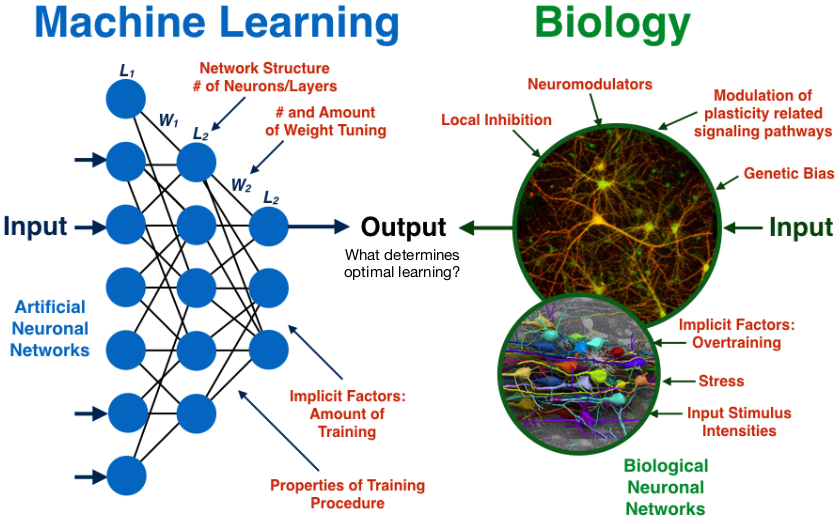
\includegraphics[width=0.8\linewidth]{01_Introduction/figures/MLvsBIO.png}
    \caption{Comparing artificial neural networks (ANNs) with biological neural networks (BNNs).}
    \label{fig:MLvsBIO}
\end{figure}
%

\subsection{Deep Learning}

\subsubsection{Applications}
\paragraph{Driving Driverless Cars:} 
Deep learning has become successful in solving tasks that were previously approached with rule based algortihms. The steering of a car is such an example. One can train a Convolutional Neural Network (CNN) to map raw pixels from a front-facing camera of a car directly to the steering commands\footnote{Bojarksi, "End to End Learning for Self-Driving Cars", 2016}.
\begin{figure}[h]
    \centering
    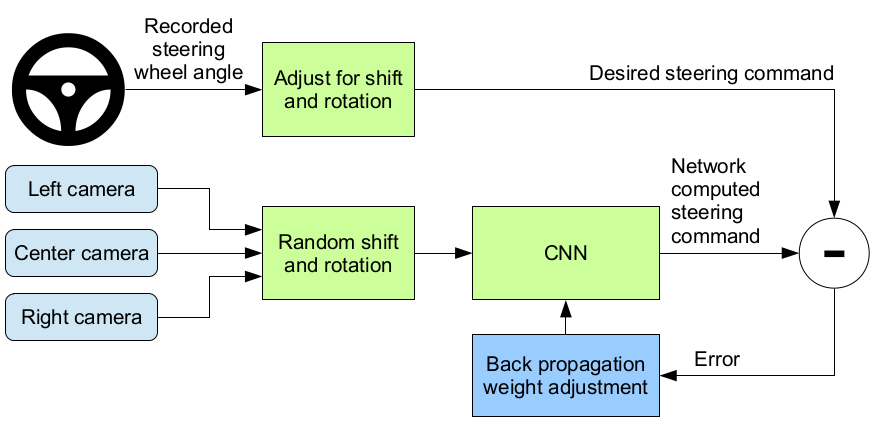
\includegraphics[width=0.6\linewidth]{01_Introduction/figures/driverless.png}
    \caption{Training of a CNN to automatically steer a car.}
    \label{fig:my_label}
\end{figure}

\paragraph{Robotic Control:}
More complex tasks, such as the actions of robotic limbs to mimic the dynamic and agile maneuvers of animals, can be approached by deep reinforcement learning\footnote{Hwangbo, "Learning Agile and Dynamic Motor Skills for Legged Robots", 2019}. 

\paragraph{Text Generation:}
Natural language processing tasks, such as question answering, machine translation, reading comprehension, and summarization, are typically approached with supervised learning on task-specific data sets. If enough data provided, they can also be approached with unsupervised deep learning \footnote{Radford, "Language Models are Unsupervised Multitask Learners", 2019}.

\paragraph{Speech Generation:}
Speech synthesis, more specifically known as text-to-speech (TTS), is a comprehensive technology that involves many disciplines such as acoustics, linguistics, digital signal processing and statistics. The main task is to convert text input into speech output.  Recent advances on speech synthesis are overwhelmingly contributed by deep learning or even end-to-end techniques which have been utilized to enhance a wide range of application scenarios such as intelligent speech interaction, chatbot or conversational artificial intelligence. For speech synthesis, deep learning based techniques can leverage a large scale of $<$text, speech$>$ pairs to learn effective feature representations to bridge the gap between text and speech, thus better characterizing the properties of events\footnote{Ning, "A Review of Deep Learning Based Speech Synthesis", 2019}.

\paragraph{Image Recognition and Med. Diagnostics:}
Deep-learning models can be trained directly on medical data to deduce patterns and thus give precise diagnostics \footnote{Using AI to predict breast cancer and personalize care: \url{http://news.mit.edu/2019/using-ai-predict-breast-cancer-and-personalize-care-0507}}.

\paragraph{Mastering Games:} 
Recently, several games that where though to be too complicated for machines to play proficiently, have been mastered by algorithms based on deep learning. One such example is the game Go. AlphaGo, a program developed by Google DeepMind, defeated the world champion in Go. The tree search in AlphaGo evaluated positions and selected moves using deep neural networks. These neural networks were trained by supervised learning from human expert moves, and by reinforcement learning from self-play \footnote{Silver, "Mastering the game of Go without human knowledge", 2017}.

\subsubsection{Challenges}\label{sec:challenges}

\paragraph{Continual learning:}
Being able to learn multiple tasks sequentially, rather than forgetting after learning a new task.
\paragraph{Robust decisions:}
Taking into account uncertainty and errors in inputs and feedback.
\paragraph{Explainable decisions:}
Understanding network reasoning and learning.
\paragraph{Security:}
Shared learning on confidential data. Look at the brain: Most of the data we perceive is not explicitly stored by the brain. 
\paragraph{Composable AI systems:}
Combining multiple systems to solve complex tasks. Look at the brain: It is comprised of over 200 different brain areas that all learn differently. 
\paragraph{Unsupervised learning:}
Learning without the need of labels by creating useful data representations. Look at the brain: It uses a combination of supervised learning, unsupervised learning and reinforcement learning\footnote{Doya, "Complementary roles of basal ganglia and cerebellum in learning and motor control", 2000}.
\begin{figure}[h]
    \centering
    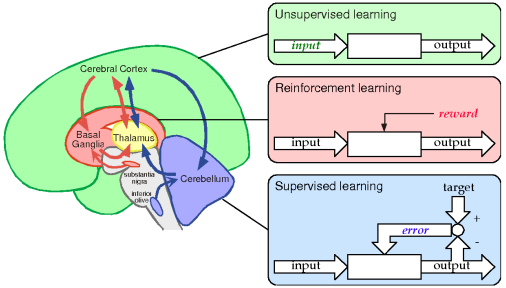
\includegraphics[width=0.5\linewidth]{01_Introduction/figures/basalandcerebellum.png}
    \caption{Supervised learning, unsupervised learning and reinforcement learning in the basal ganglia and the cerebellum.}
    \label{fig:basalandcerebellum}
\end{figure}


\paragraph{Fast learning:} 
Using only a few data examples to create generalizing representations. Look at the brain: It seems to learn from extremely few examples.

\subsection{The Human Brain as Universal Learning Machine}

\paragraph{Universal Learning Machine (ULM):} A simple and yet very powerful and general model for intelligent agents\footnote{Cool blog post: \url{https://www.lesswrong.com/posts/9Yc7Pp7szcjPgPsjf/the-brain-as-a-universal-learning-machine}}. It is an extension of a general computer - such as Turing Machine - amplified with a universal learning algorithm. An initial untrained seed ULM can be defined by 1.) a prior over the space of models (or equivalently, programs), 2.) an initial utility function, and 3.) the universal learning machinery/algorithm.  The machine is a real-time system that processes an input sensory/observation stream and produces an output motor/action stream to control the external world using a learned internal program that is the result of continuous self-optimization. 


\paragraph{Inheritance:} One criticism to typical artificial neural networks (ANNs) and supervised learning in general is, that everything is learned and nothing inherited. Contrarily, young animals (including humans) learn without seeing an enormous numbers of labeled examples. This could either lead to the belief, that animals must rely on unsupervised learning, or that most animal behavior is actually encoded in the genome. Specifically, animals are born with highly structured brain connectivity, which enables them to learn very rapidly. Because the wiring diagram is far too complex to be specified explicitly in the genome, it must be compressed through a “genomic bottleneck”. The genomic bottleneck suggests a path toward ANNs capable of rapid learning\footnote{Zador, "A critique of pure learning and what artificial neural networks can learn from animal brains", 2019}. There are animals, such as the simple worm \textit{C. Elegans}, stores the entire neuronal wiring in its genome. Thus, the wiring pattern is identical for each worm. 

\paragraph{The human brain in numbers:} At 1232 grams, the human brain has about $10^{11}$ neurons, and more than $10^3$ synapses per neuron. Specifying a connection target requires about $\log_2 10^{11}$ = 35 bits/synapse. Thus it would take about $3.5 * 10^{15}$ bits ($\approx 400$ TB) to specify all $10^{14}$ connections in the brain. One could therefore conclude, that the human brain is mostly learned.

\paragraph{Artificial General Intelligence (AGI):} The intelligence of a machine that could successfully learn and perform any intellectual task similar to a human.

\newpage
\subsection{The Mammalian Neocortex}
\begin{figure}[h]
    \centering
    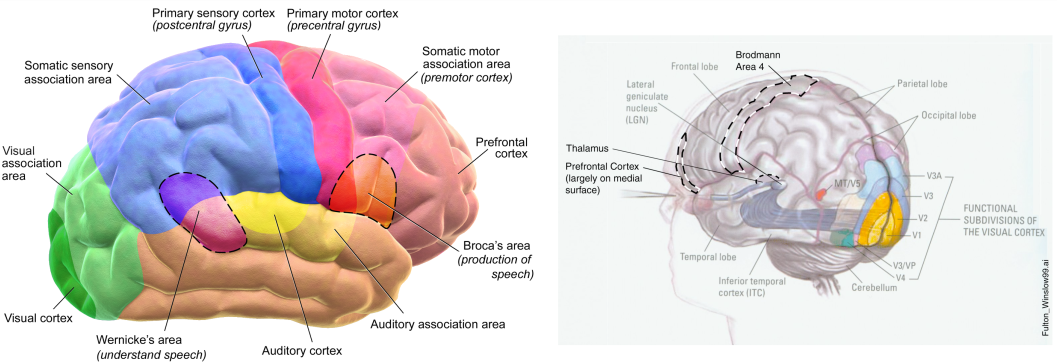
\includegraphics[width=0.99\linewidth]{01_Introduction/figures/neocortex.png}
    \caption{Illustration of the mammalian neocortex}
    \label{fig:basalandcerebellum}
\end{figure}

\subsubsection{Key Facts}
The neocortex is ...
\begin{itemize}
    \item the top layer of the cerebral hemispheres, 2-4 mm thick, and made up of six layers, labelled I to VI.
    \item part of the cerebral cortex (along with the archicortex and paleocortex, which belong to the limbic system).
    \item involved in higher functions such as sensory perception, generation of motor commands, spatial reasoning, conscious thought, and language.
    \item consists of grey matter surrounding the deeper white matter of the cerebrum.
    \item smaller and smoother in rats and some other small mammals, but it has deep grooves (sulci) and wrinkles (gyri) in primates and several other mammals. These folds serve to increase the area of the neocortex considerably.
    \item accounting for about 76\% of the brain's volume of humans.
\end{itemize}

\subsubsection{The 6 Layers of the Mammalian Neocortex}
\begin{figure}[H]
    \centering
    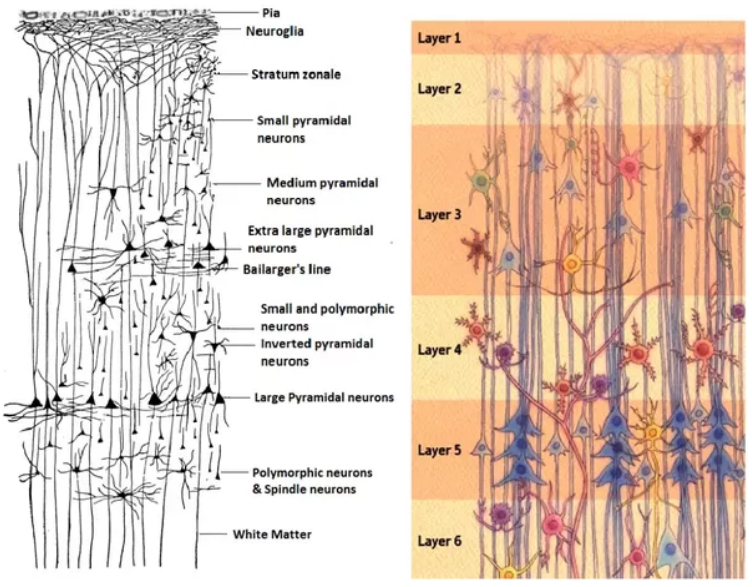
\includegraphics[width=0.8\linewidth]{01_Introduction/figures/layers_illustrated.png}
    \caption{Caption}
    \label{fig:basalandcerebellum}
\end{figure}

\begin{figure}[H]
    \centering
    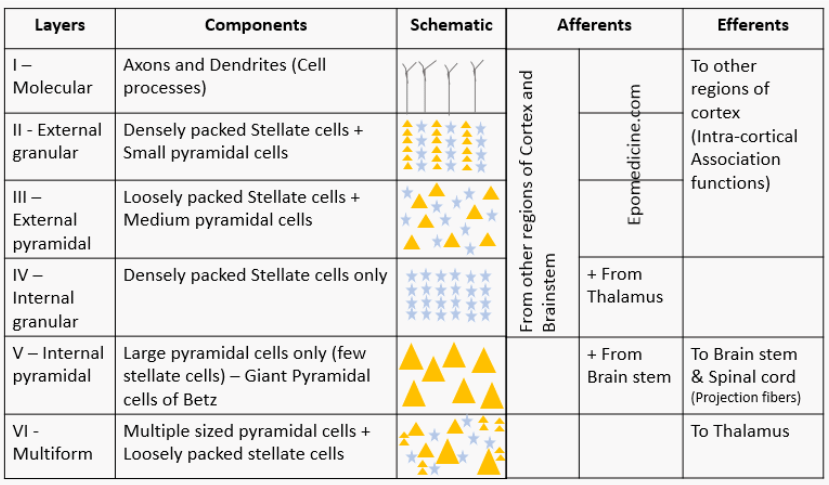
\includegraphics[width=0.95\linewidth]{01_Introduction/figures/layers_table.png}
    \caption{Caption}
    \label{fig:basalandcerebellum}
\end{figure}

\subsubsection{Visual Apparatus}

\begin{figure}[H]
    \centering
    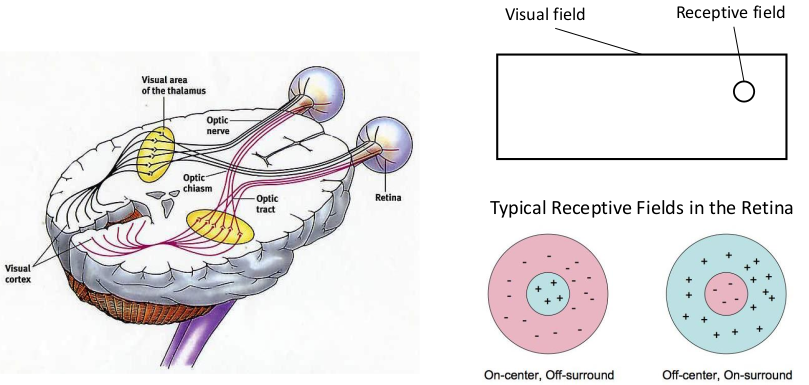
\includegraphics[width=0.8\linewidth]{01_Introduction/figures/visual_apparatus.png}
    \caption{}
    \label{fig:basalandcerebellum}
\end{figure}

\begin{figure}[H]
    \centering
    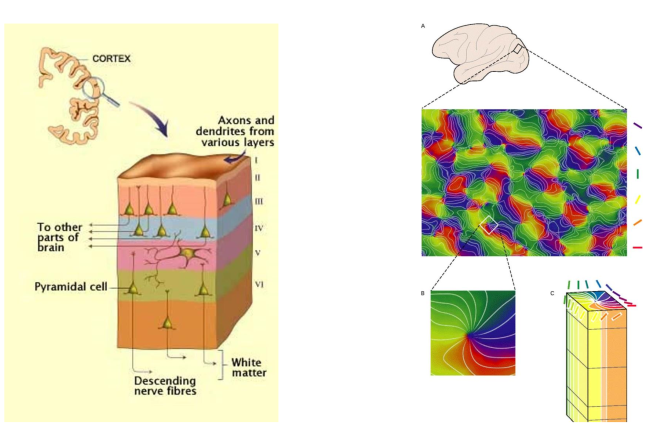
\includegraphics[width=0.8\linewidth]{01_Introduction/figures/layers_orientation.png}
    \caption{}
    \label{fig:basalandcerebellum}
\end{figure}

\subsubsection{Hubel and Wiesel Experiment}
The Hubel and Wiesel experiments greatly expanded the scientific knowledge of sensory processing. In one experiment, done in 1959, they inserted a microelectrode into the primary visual cortex of an anesthetized cat. They then projected patterns of light and dark on a screen in front of the cat. They found that some neurons fired rapidly when presented with lines at one angle, while others responded best to another angle. Some of these neurons responded differently to light patterns than to dark patterns. Hubel and Wiesel called these neurons "simple cells." Still other neurons, which they termed "complex cells," had identical responses to light and dark patterns. These studies showed how the visual system constructs complex representations of visual information from simple stimulus features\footnote{Goldstein, 2001} \footnote{\url{https://www.brains-explained.com/how-hubel-and-wiesel-revolutionized-neuroscience/}}, \footnote{Wiesel, "Eye, Brain, and Vision", 1988}.

\begin{figure}[H]
    \centering
    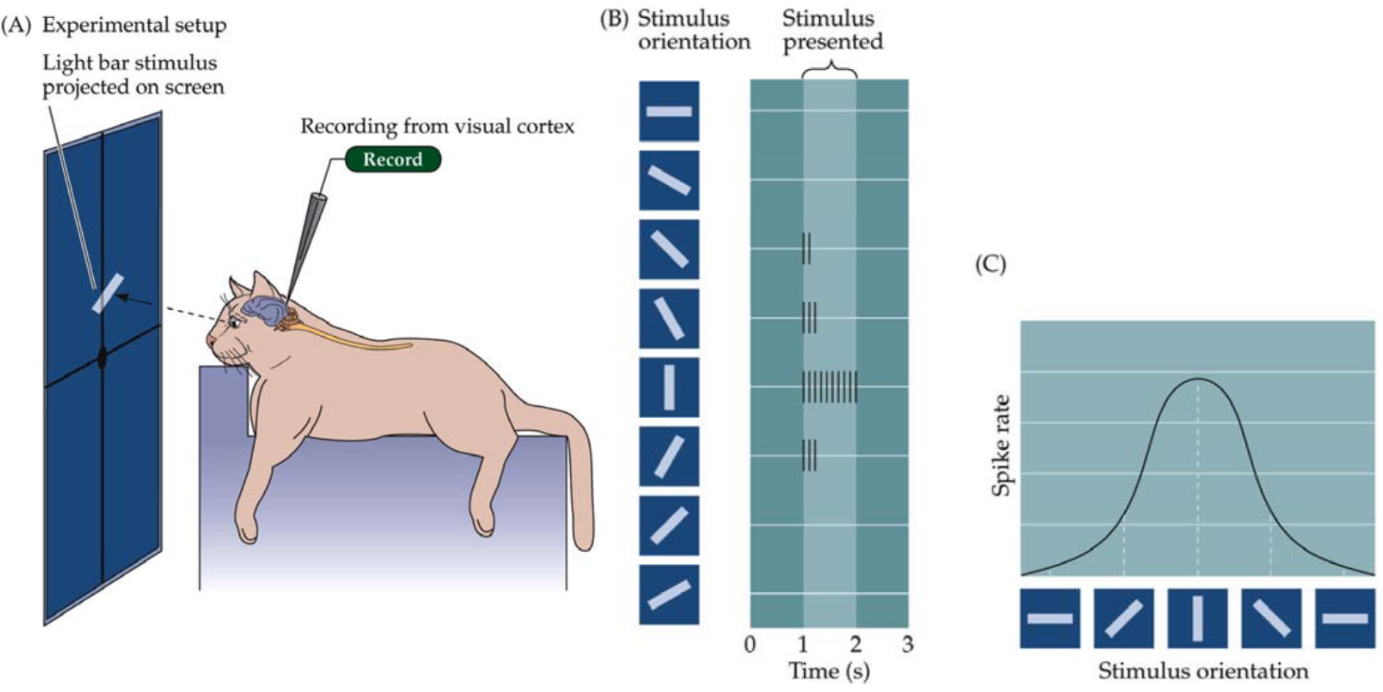
\includegraphics[width=0.8\linewidth]{01_Introduction/figures/hubelwieselexperiment.png}
    \caption{\textbf{A:} Hubel and Wiesels cat experiment. \textbf{B\&C:} Orientation and direction selectivity in cortical neurons}
    \label{fig:basalandcerebellum}
\end{figure}

\begin{figure}[H]
    \centering
    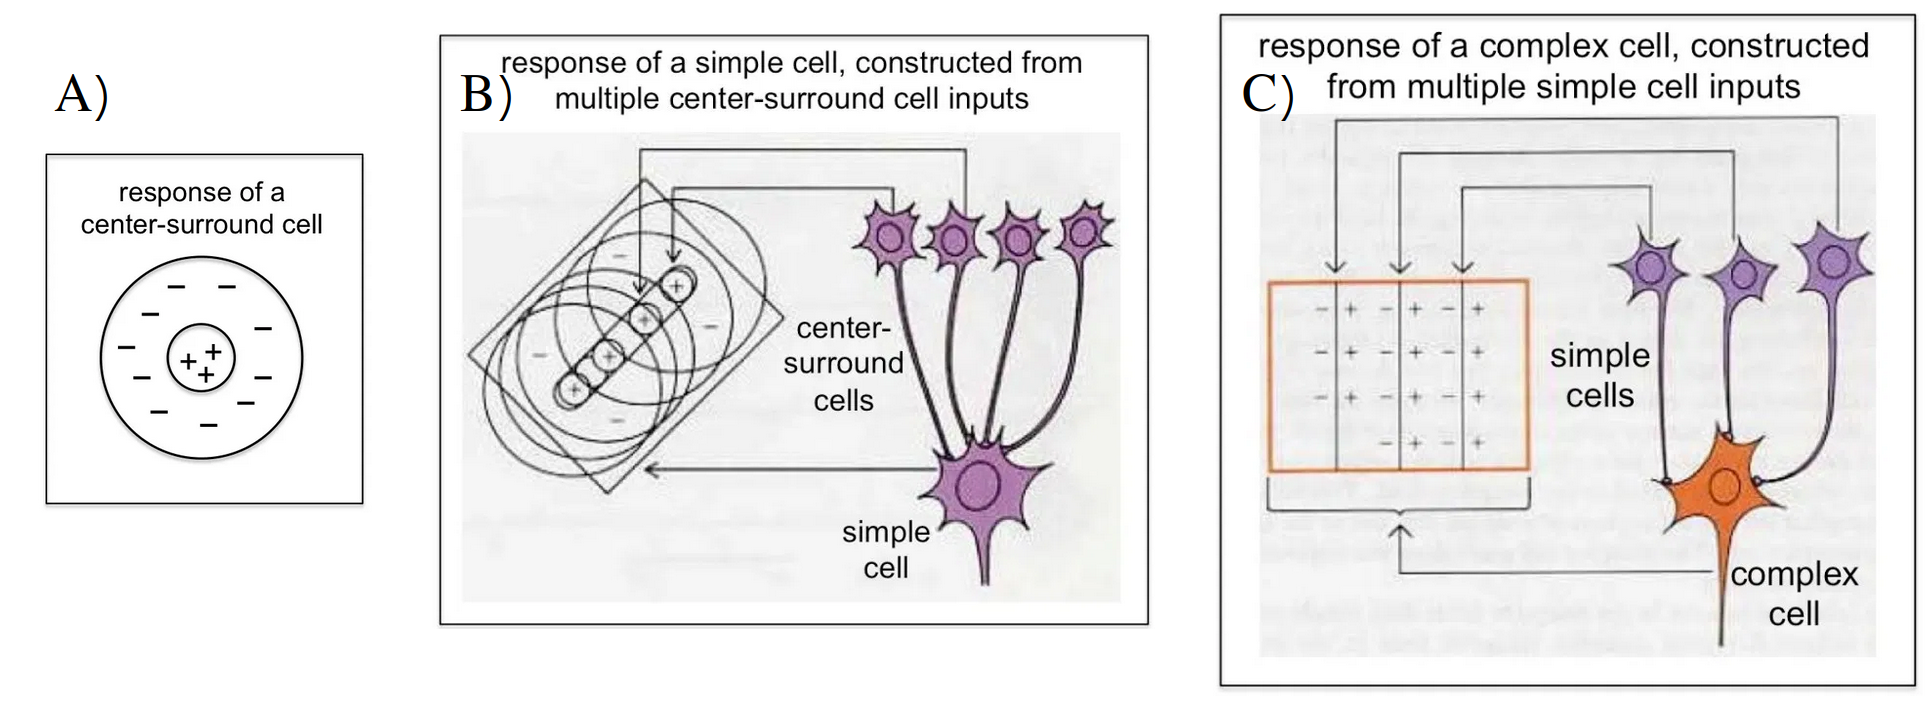
\includegraphics[width=0.9\linewidth]{01_Introduction/figures/hubelwieselresults.png}
    \caption{\textbf{A:} Depiction of center-surround cell responses. This cell is excited by light presented in a small, circular central area (plus signs) and inhibited by light in the surrounding area (minus signs). \textbf{B:} The simple cell receives input from multiple center-surround cells whose preferred areas (small circles with plus signs) are aligned in a straight line. The larger circles with minus signs again depict how light in the surrounding area inhibits the cells. \textbf{C:} A complex cell receives input from multiple simple cells that respond to lines of the same orientation (in this case, vertical) but positioned adjacently. (Plus and minus signs depict how simple cells are excited by a line in one position but inhibited by a line in an adjacent position, similar to center-surround cells. This explains why a large shape like a square won’t activate the complex cell- it would trigger too much inhibition.}
    \label{fig:basalandcerebellum}
\end{figure}

\subsection{Parallels and differences between artificial and biological networks}
\subsubsection{McCulloch and Pitts Neuron and the Perceptron}
The McCulloch and Pitts Neuron is a highly simplified computational model of the cortical neuron. Excitatory or inhibitory inputs are aggregated; an output is produced if the aggregation reaches a certain (adjustable) threshold. The MCP takes boolean inputs only. 

The Perceptron is very similar to the MCP, but it takes real valued inputs, which are weighted. Both models are linear, but by accumulating multiple units, one can achieve non-linear separation\footnote{\url{https://medium.com/analytics-vidhya/mp-neuron-and-perceptron-model-with-sample-code-c2189edebd3f}}. 

\begin{figure}[H]
    \centering
    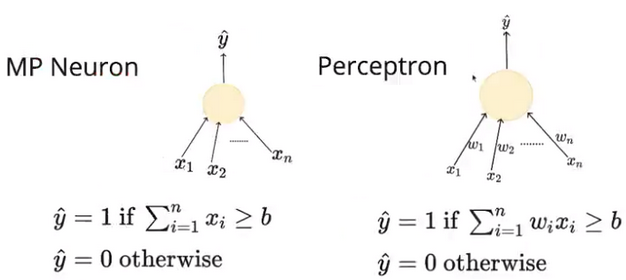
\includegraphics[width=0.8\linewidth]{01_Introduction/figures/MCP_Perceptron.png}
    \caption{Comparing the MCP and the Perceptron}
    \label{fig:basalandcerebellum}
\end{figure}

\subsubsection{Hierarchical Models}
\begin{figure}[H]
    \centering
    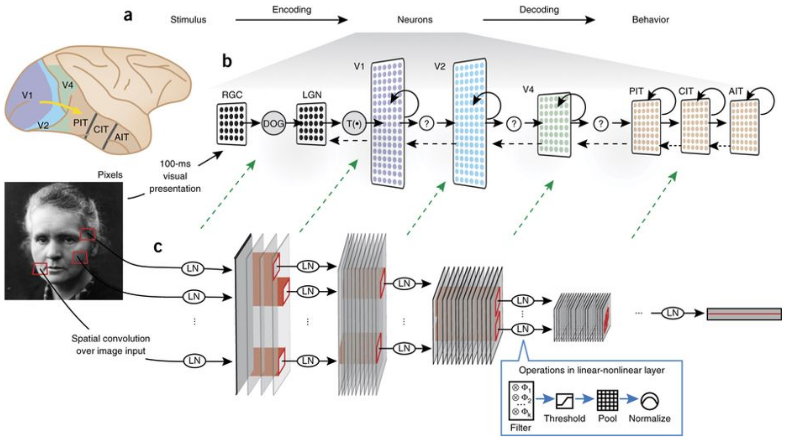
\includegraphics[width=0.99\linewidth]{01_Introduction/figures/hierarchical.png}
    \caption{}
    \label{fig:basalandcerebellum}
\end{figure}

\subsubsection{Parallels}
How is information processing and learning in deep networks and biological networks similar?

\subsubsection{Differences}
How does information processing and learning in deep networks and biological networks differ?


\subsection{Experimental Methods in Neuroscience}
\paragraph{Electrophysiology} is the branch of physiology that studies the electrical properties of biological cells and tissues. It involves measurements of voltage changes or electric current or manipulations on a wide variety of scales from single ion channel proteins to whole organs like the heart. In neuroscience, it includes measurements of the electrical activity of neurons, and, in particular, action potential activity\footnote{\url{https://en.wikipedia.org/wiki/Electrophysiology}}.

\begin{figure}[H]
    \centering
    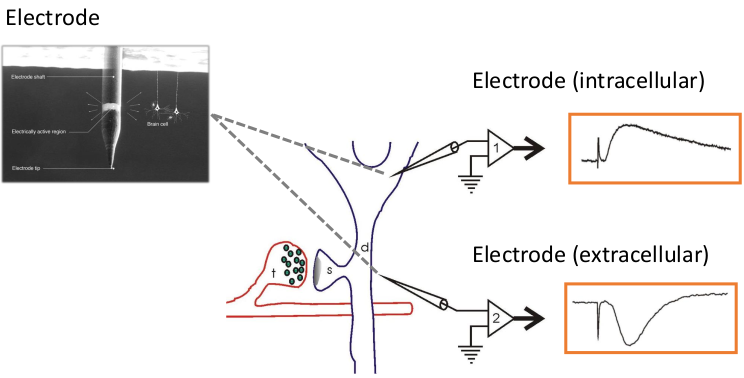
\includegraphics[width=0.99\linewidth]{01_Introduction/figures/electrophysiology.png}
    \caption{}
    \label{fig:basalandcerebellum}
\end{figure}


\paragraph{Calcium Imaging} is a indirect measurement method which is designed to show the calcium (\ce{Ca^2+}) status of an isolated cell, tissue or medium. Calcium imaging techniques take advantage of so-called calcium indicators, fluorescent molecules that can respond to the binding of Ca2+ ions by changing their fluorescence properties. Two main classes of calcium indicators exist: chemical indicators and genetically encoded calcium indicators (GECI). Calcium imaging can be used to optically probe intracellular calcium in living animals. This technique has allowed studies of calcium signalling in a wide variety of cell types and neuronal activity in hundreds of neurons and glial cells within neuronal circuits\footnote{\url{https://en.wikipedia.org/wiki/Calcium_imaging}}. 


\paragraph{Functional Magnetic Resonance Imaging (fMRI)} indirectly measures brain activity by detecting changes associated with blood flow. This technique relies on the fact that cerebral blood flow and neuronal activation are coupled. When an area of the brain is in use, blood flow to that region also increases. The primary form of fMRI uses the blood-oxygen-level dependent (BOLD) contrast\footnote{\url{https://en.wikipedia.org/wiki/Functional_magnetic_resonance_imaging}}.

\subsection{Questions}
\begin{enumerate}
    \item What is the duration of a spike?
    \item How fast do APs propagate along the axon?
\end{enumerate}

\end{document}